\chapter{Literature Review}\label{LiteratureReview}
For this dissertation, research was conducted to find the most recent trends in 2D fluid segmentation of OCT volumes using deep learning and in the use of generative models in the intermediate slice synthesis.
\section{Fluid Segmentation}
In the fluid segmentation state-of-the-art research, articles were retrieved using the methodology of a systematic review. The next subsection details the retrieval process and the criteria for inclusion and exclusion of the articles. ``\ref{FluidSegmentationLiteratureReview} Literature Review" shows the trends on the methodologies utilized for fluid segmentation.
\subsection{Search Strategy}\label{SearchStrategy}
The search query was defined as: ````OCT" AND ``segmentation" AND (``deep learning" OR ``CNN" OR ``neural network")". Using the query, papers were retrieved from four different databases: 398 articles from PubMed, 105 from IEEE, 125 from ScienceDirect, and 80 from ACM.
\par
In the process of collecting the papers, those published over the previous five years and regarding 2D or 2.5D fluid segmentation in OCT volumes were included. Additionally, conferences proceedings, articles not written in English, and articles for which the full text was not accessible were excluded.
\par
A total of 708 articles were initially identified, of which 133 were duplicates. Afterwards, 575 articles were subjected to screening, based on their titles and abstracts. These articles were analyzed in accordance with the inclusion and exclusion criteria, resulting in the removal of 499 papers. Of the remaining 76 articles for the full-text screening, 20 met the established criteria. These final articles represent the state-of-the art in 2D deep learning fluid segmentation in OCT volumes included in this dissertation.

\subsection{Literature Review}\label{FluidSegmentationLiteratureReview}
The selected papers \cite{Pawan2021, Liu2021, Guo2020, Wu2023, Wang2021, Quek2022, Mantel2021, Li2023, Hassan2021a, Padilla2022, Liu2024, Zhang2023, Tang2022, Xing2022, Rahil2023, Lu2019, Hassan2021b, Hu2019, Sappa2021, Gao2019} can be divided into two broad groups, according to the type of segmentation: binary segmentation \cite{Quek2022, Pawan2021, Liu2021, Guo2020, Wang2021, Wu2023}, where the fluid is classified in one whole class, and multi-class \cite{Rahil2023, Hassan2021a, Zhang2023, Sappa2021, Xing2022, Tang2022, Padilla2022, Hu2019, Mantel2021, Liu2024, Li2023, Gao2019, Hassan2021b, Lu2019}, where the segmented fluid is classified in two or more classes (namely IRF, SRF, and PED). We have also considered other criteria to group the papers, such as the segmentation architecture, and the use of retinal delimitation, as shown in Figure \ref{fig:ArticlesSelection}.
\par
In binary segmentation, the approaches to the segmentation problem are simpler, but include both convolutional neural network (CNN) \cite{Pawan2021, Liu2021, Guo2020, Wang2021, Wu2023} and transformer solutions \cite{Quek2022}. The CNN solutions differ among them, depending on the modules that constitute each network, but all are inspired by the U-Net \cite{Ronneberger2015}. In Figure \ref{fig:BinarySegmentationExample}, an instance of a CNN used for binary fluid segmentation is shown.
\begin{figure}[!ht]
	\centering
	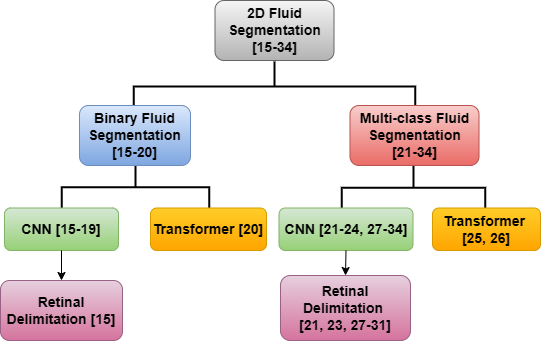
\includegraphics[width=0.75\linewidth]{../figures/ArticlesSelection.png}
	\caption{Grouping of the articles included in the literature review.}
	\label{fig:ArticlesSelection}
\end{figure}
\begin{figure}[!ht]
	\centering
	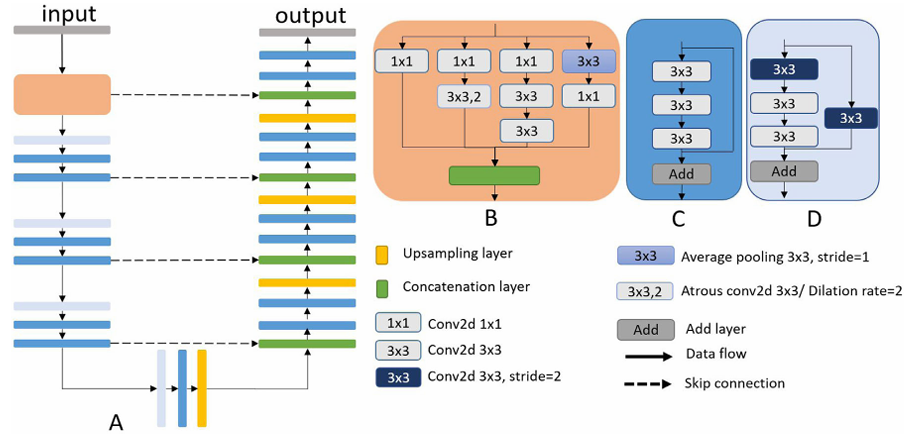
\includegraphics[width=1\linewidth]{../figures/BinarySegmentationExample.png}
	\caption{Example of a CNN architecture used in fluid binary segmentation. Image A depicts the neural network architecture. B shows the used multi-scale block, while C and D exhibit the residual convolutional blocks \cite{Guo2020}.}
	\label{fig:BinarySegmentationExample}
\end{figure}
\par
Pawan \textit{et al}. \cite{Pawan2021} is the only paper in binary segmentation that restricts the input of the segmentation CNN to the content within the retinal layer. This approach is frequently observed in the papers focused on multi-class segmentation. In this paper, this is achieved by performing a retinal layer segmentation and assigning all the values outside the boundaries to zero. The result of this operation is an input for the segmentation CNN. The removal of irrelevant information surrounding the retina simplifies the learning process and improves the model's focus on essential information \cite{Mantel2021}.
\par
In the framework proposed by Liu \textit{et al}. \cite{Liu2021}, the  slice's fluid mask and distance map are generated. The distance map consists of the predicted distance of each pixel to the background or retinal tissue, with only the values above a specified distance threshold being kept. This is achieved through the use of a double-branched network, where the encoder is the same, while the decoders vary. One encoder is responsible for generating the fluid segmentation map, while the other predicts the distance map. The intersection between these outputs forms the final segmentation. This approach mitigates the issue of inappropriate merging of small and proximate fluid regions, as the distance branch is better than the fluid segmentation network in discerning the boundaries that delineate fluid regions.
\par
Resorting to generative adversarial networks (GANs), Wu \textit{et al}. \cite{Wu2023} make images from different vendors, visually similar to the images of a singular, specific vendor. Subsequently, a U-Net, which has extensively been trained on images from the specific vendor, is used for segmentation. This approach is intended to reduce the burden of learning the segmentation on multiple vendors by ensuring that all volumes are similar to one in which the segmentation model performs well. Similarly, the multi-class segmentation framework proposed by Li \textit{et al}., 2023 \cite{Li2023} was designed based on the same idea. 
\par
CNNs inspired by the U-Net can also be combined with transformers in the context of image segmentation. While CNNs capture the information from local receptive fields, visual transformers integrate features from global receptive fields. Despite being more prevalent in multi-class segmentation frameworks, in this paper by Quek \textit{et al}. \cite{Quek2022}, the visual transformers are located between the encoder and decoder paths, thus incorporating features from both receptive fields in the encoding branch.
\par
The majority of the papers included in this review perform multi-class segmentation models, therefore presenting more diverse implementations. While all the articles here considered segment two or more fluids, Hassan \textit{et al.} (2021) \cite{Hassan2021a} and Padilla-Pantoja \textit{et al.} (2022) \cite{Padilla2022} also segment other biomarkers. Similarly to binary segmentation, the multi-class segmentation papers can also be divided according to the presence \cite{Zhang2023, Liu2024} or absence \cite{Rahil2023, Hassan2021a, Sappa2021, Xing2022, Tang2022, Padilla2022, Hu2019, Mantel2021, Li2023, Gao2019, Hassan2021b, Lu2019} of transformers in the segmentation network. All the papers that have transformers in their framework, combine them with CNNs. 
\par
Similar to what was developed in \cite{Quek2022}, Liu \textit{et al}. (2024) \cite{Liu2024} have integrated transformers in the bottleneck section of a segmentation network inspired by the U-Net. \cite{Liu2024} utilize two networks for the segmentation: one for coarse segmentation and other for the refinement of the results from the first. Both networks are similar to the U-Net, but in the refine branch, a transformer is included. Its purpose is to provide features from global fields, compensating for the deep features that are used as input in this branch. In contrast, Zhang \textit{et al}. \cite{Zhang2023} replaced the CNN encoder with a transformer encoder, exploiting its modeling capacity with self-attention.
\par
The limitation of the input to the region within the retinal layer, ignoring what is outside of it, is seen in many of the multi-class papers \cite{Hassan2021b, Hassan2021a, Lu2019, Mantel2021, Rahil2023, Tang2022, Xing2022}, similarly to what was done in \cite{Pawan2021}. There are various approaches for this delimitation, with some using CNNs trained for the segmentation of the retinal layers or the retina \cite{Mantel2021, Tang2022}, and others using algorithms leveraging on the noticeable transition between the retinal layers and its background \cite{Hassan2021b, Hassan2021a, Lu2019, Rahil2023, Xing2022, Pawan2021}. 
\par
The retinal delimitation is conducted as a separate process from the fluid segmentation. In \cite{Tang2022, Hassan2021b, Hassan2021a, Lu2019, Rahil2023, Xing2022}, the retinal layer is segmented prior to the fluid segmentation, conditioning the input of the fluid segmentation network and simplifying the learning process. However, the retinal delimitation can also limit the final segmentation by intersecting the network's output, limiting the segmentation results to the boundaries of the retinal layer, as observed in \cite{Mantel2021}.
\par
The fluid segmentation network input is conditioned in multiple ways. In \cite{Xing2022}, the image is cropped to fit its region of interest. \cite{Rahil2023, Tang2022, Lu2019} combined the B-scan with the retinal delimitation result, either through concatenation or along another channel. In \cite{Hassan2021b, Hassan2021a, Pawan2021} the information outside the retinal layer is set to zero and ignored. 
\par
Contrasting with the work of Liu \textit{et al}. \cite{Liu2021} who used a CNN to output a distance map (relative to the background or the retinal tissue), \cite{Tang2022} and \cite{Rahil2023}, inspired by the work of \cite{Lu2019}, calculate a relative distance map to combine with the input slice in a CNN. Starting with the retinal delimitation, the relative distance to the internal limiting membrane (ILM) is calculated for each pixel located between the ILM and the Bruch's membrane (BM) (see Figure \ref{fig:RetinalLayers}). This map provides information about the relative position of each pixel to the ILM, influencing their classification. An example of such framework can be seen in Figure \ref{fig:PreSegmentationAndFluidSegmentation}.
\par
\begin{figure}[!ht]
	\centering
	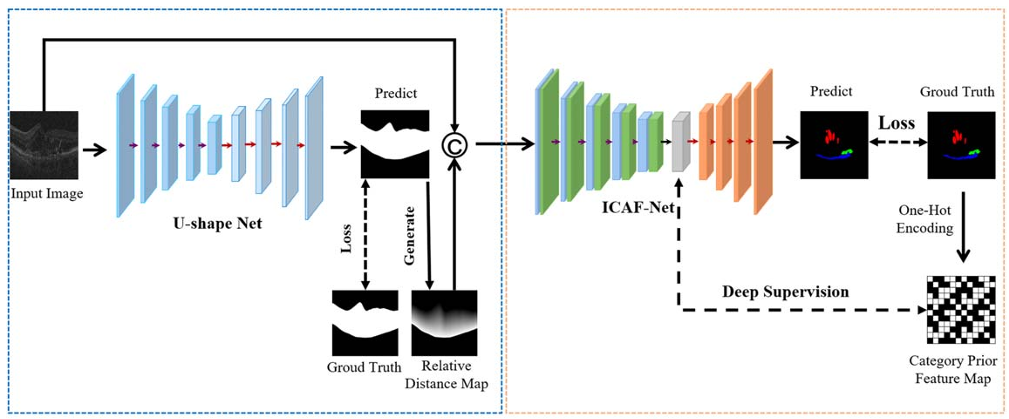
\includegraphics[width=1\linewidth]{../figures/PreSegmentationAndFluidSegmentation.png}
	\caption{Example of a framework that includes delimitation of the retinal layer and a relative distance map (left side). The generated map is included in the segmentation network (denominated ICAF-Net, by the authors) \cite{Tang2022}.}
	\label{fig:PreSegmentationAndFluidSegmentation}
\end{figure}
\par
Regarding the segmentation CNNs adopted by the analyzed papers, most are directly inspired by the U-Net, to which changes are done, when considering the objectives of each study. Examples of such changes are the introduction of blocks (such as residual \cite{Mantel2021, Zhang2023, Liu2024, Hassan2021b, Hassan2021a, Padilla2022}), and modules (like atrous sampling pyramid pooling \cite{Hassan2021b, Hassan2021a, Hu2019, Sappa2021}), which makes the network distinctive. However, some papers use other variations of the U-Net that are also popular: the Deeplab \cite{LChen2018} in \cite{Hassan2021a, Li2023} and the VGG \cite{Simonyan2014} in \cite{Padilla2022, Hassan2021b}.

\section{Intermediate Slice Synthesis}
For many years, there have been attempts to improve the resolution of OCT exams using computational methods, a process called super-resolution (SR). In 3D applications, such as magnetic resonance imaging (MRI), computed tomography (CT), and OCT, SR can be done intra-slice, which improves the resolution of each slice in the volume along one plane, or inter-slice, bettering the resolution of the volume along one axis, by generating one or more slices between a pair of original ones. Some frameworks may contain both approaches \cite{You2020}.
\par
The use of GANs to generate slices between other known slices is commonly used technique in MRI and CT, but with few examples in OCT \cite{You2020}. The systematic literature review performed by Ibrahim \textit{et al}. (2024) \cite{Ibrahim2024}, which analyzed the latest trends in the use of generative models in medical data, only presents one example of GAN for inter-slice resolution improvement in OCT volumes \cite{Lopez2023}. In this imaging technique, the use of GANs is mainly done for the generation of OCT images and conversion between different vendors \cite{Ibrahim2024}.
\par
In the following subsection, the state-of-the-art architectures used for the improvement of inter-slice resolution are presented.

\subsection{Architectures}
Given the lack of examples in OCT imaging, it was considered appropriate to study works from other imaging techniques, given that the working principle is the same across them. The selected papers can be classified into three distinct categories: inter-slice SR, which leverages information from adjacent slices to generate one or more intermediate slices \cite{Lopez2023, Xia2021, Wu2022, Nishimoto2024}; intra-slice SR combined with inter-slice SR, which improves the resolution of the slices from orthogonal planes and combines them with the results of inter-slice SR \cite{Zhang2024, Fang2022, Nimitha2024, Georgescu2020}; and SR applied directly in 3D volumes, utilizing three-dimensional convolutions in the generation process, which incorporates the information along all the axes from multiple slices simultaneously \cite{YChen2018, Sanchez2018, Kudo2019, Zhang2022}.
\par
In \cite{Lopez2023}, López-Varela \textit{et al}. present an inter-slice SR framework based on a GAN (inspired by the ResNet) for the generation of three B-scan slices between two known slices. The GAN training process, as illustrated in Figure \ref{fig:GANGenerationFramework}, begins with the generation of an intermediate slice (Central Fake) located between two original B-scans (Pre and Post), which are separated by another original one (Central). The Central B-scan will serve as the ground truth (GT) and will be used for the assessment of image quality generated by the network. Subsequently, the network generates other two slices: one between the Pre and Central slices, designated as Pre-Central fake, and another between the Central and Post slices, named Post-Central fake. As the mentioned generations lack a corresponding GT, the network performance is regulated by using these two new synthetic slices to generate an additional Central Fake (Central Fake 2), which is then compared to the true Central. Consequently, if the generation of Pre- and Post-Central fakes are inadequate, the Central Fake 2 will also be of poor quality, resulting in a higher loss value. During the inference process, one slice is synthesized for every two known B-scans, reducing the inter-slice distance to half of the original value.
\par
The importance of this study comes not only from it being the only study in OCT but also from the approach selected, which is similar to the foundation of the frameworks implemented in other papers. 

\begin{figure}[!ht]
	\centering
	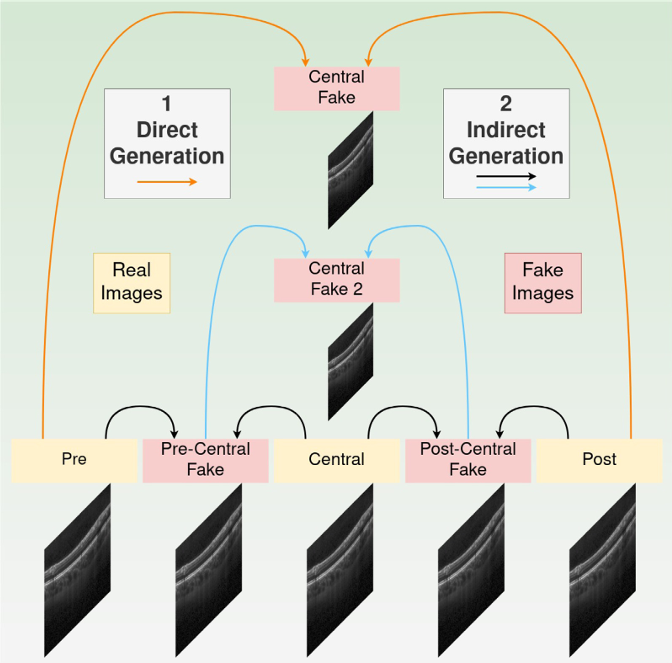
\includegraphics[width=0.75\linewidth]{../figures/GANGenerationFramework.png}
	\caption{López-Varela \textit{et al}. \cite{Lopez2023} training process.}
	\label{fig:GANGenerationFramework}
\end{figure}

In a more straightforward approach, Nishimoto \textit{et al.}, 2024 \cite{Nishimoto2024} utilize a baseline U-Net that uses two spaced slices as input to generate the slices between them. This methodology was tested in the generation of three, four, and five intermediate slices, and obtained better outcomes than those generated through linear interpolation.
\par
The work by Xia \textit{et al}. \cite{Xia2021} demonstrates the enhancement of inter-slice resolution in MRI, through the utilization of multiple networks and a multi-scale discriminator that considers both the image from a large and a small field of view images. Additionally, the framework also estimates the depth and flow of each pair of images, generating an independent image from the GAN. This subsequently facilitates the generation of the intermediate slice.
\par
Similarly, Wu \textit{et al}. \cite{Wu2022} improved the inter-slice resolution by training a single GAN to generate bi-directional spatial transformations instead of producing fake images. The advantage of this process is that it allows the same transformations to be applied to the segmentation masks from the surrounding slices, generating fake masks for the fake slices. As in \cite{Xia2021}, the discriminator also judges the generated images in both a larger and smaller field of view, but combines this with an object classifier that checks if the structures present in the neighboring slices appear in the fake one.
\par
As an example of the use of intra-slice SR to improve inter-slice resolution, Zhang \textit{et al}. \cite{Zhang2024} implemented two GANs that increase the resolution in the slices of the two planes with the lowest resolution of the volume (sagittal and coronal). In these planes, the dimensions of each slice are increased in the direction of the axis of lowest inter-slice resolution. Simultaneously, in the plane of highest resolution (axial), an architecture similar to López-Varela \textit{et al}. (2023) \cite{Lopez2023} is used in the generation of intermediate fake slices between each pair of known slices. The results from these three networks are then compared between each other, promoting the accurate and consistent generation of data among the networks.
\par
A similar approach was done by Fang \textit{et al}. \cite{Fang2022}, in which three networks (one for each axis) are trained to generate intermediate slices along one axis with a lower inter-slice resolution. However, during the unsupervised phase, upon each increase in resolution (a process that occurs twice), the information generated by the networks is compared between each other and a loss value that quantifies the performance is calculated, as illustrated in Figure \ref{fig:FangArchitecture}.
\begin{figure}[!ht]
	\hspace*{-0.7in}
	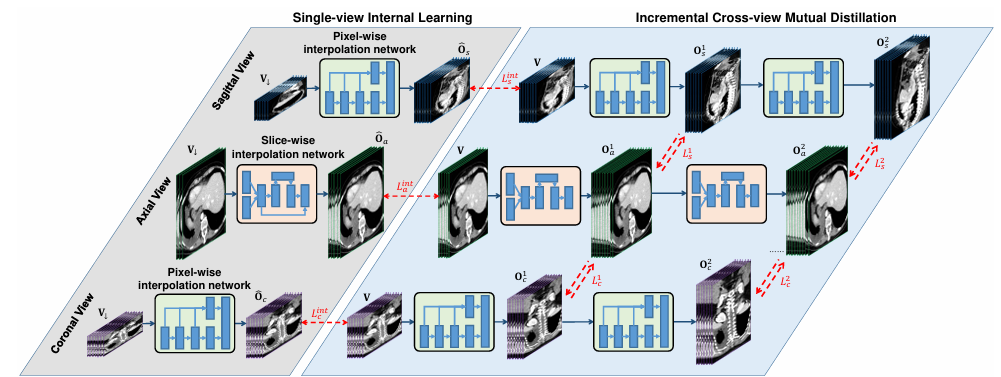
\includegraphics[width=1.25\linewidth]{../figures/FangArchitecture.png}
	\caption{Pipeline of the methodology utilized by Fang \textit{et al}., 2022 \cite{Fang2022}.}
	\label{fig:FangArchitecture}
\end{figure}
\par
Similarly, Nimitha and Ameer (2024) \cite{Nimitha2024} use GANs to improve intra-slice resolution and a CNN to improve inter-slice resolution. The method starts by increasing the resolution of low-resolution (LR) slices, making them high-resolution (HR). Then an intermediate HR slice is generated between every set of two slices, using a CNN.
\par
The same approach was also used by Georgescu \textit{et al.}, 2020 \cite{Georgescu2020} to enhance the intra- and inter-slice resolution in CT and MRI scans. Two independently trained CNNs were used in LR volumes. One CNN was tasked with generating HR slices from the LR slices. Concurrently, the other CNN was utilized to reduce the distance between slices by increasing the resolution of the images from the orthogonal plane. By inferring an image with increased resolution along this plane, new intermediate slices were generated, improving the inter-slice resolution along the low resolution axis.
\par
The methodologies utilizing 3D GANs are similar between each other, as they all apply networks based on the GANs implemented in 2D images. As this method already considers the information across all the axes simultaneously, there is no need to use multiple networks for each, as seen in some of the previous approaches. Therefore, the differences between papers mainly originate from the medical imaging technique to which it is applied, the modules that constitute the 3D GANs used, and the datasets used for evaluation \cite{YChen2018, Sanchez2018, Kudo2019, Zhang2022}.
